\nocite{MathWorksParallelComputing}
Il \textit{Parallel Computing Toolbox}, spesso abbreviato in PCT, permette di risolvere problemi \textit{compute-intesive} e  \textit{data-intensive} sfruttando 
la capacit\`a di calcolo offerta dalle moderne architetture multiprocessore, come i sistemi \textit{multicore} e i \textit{cluster} di elaboratori. \newline
Costrutti di programmazione di alto livello, come i vettori distribuiti, consentono di sviluppare applicazioni MATLAB scalabili senza ricorrere alla programmazione 
MPI \footnote{La \textit{Message Passing Interface}, o semplicemente MPI, rappresenta lo standard per il modello di comunicazione interprocesso, basato sullo scambio 
di messaggi, impiegato nelle elaborazioni parallele su sistemi distribuiti \cite{NMSUMPIIntro}}.\newline
Inoltre, la stessa applicazione pu\`o essere eseguita su \textit{cluster} o su server in \textit{cloud} senza apportare alcuna modifica al codice grazie a MATLAB 
\textit{Parallel Server}, cos\`i da concentrarsi esclusivamente sullo sviluppo dell'algoritmo migliore per il caso d'uso in esame.

Incominciamo il nostro studio del PCT riportando alcune definizioni, tratte dalla documentazione ufficiale di MATLAB \cite{MathWorksWhatIsParallel}, di aspetti del modello di programmazione parallela fondamentali per la prosecuzione della trattazione.
\begin{itemize}
\item \textit{Client}: termine impiegato per identificare la sessione di MATLAB attiva con cui l'utente finale sta interagendo; tipicamente coincide con il 
\textit{computer} usato dallo sviluppatore durante la prototipazione e lo sviluppo in locale del programma a esecuzione parallela.\newline
Attraverso le funzionalit\`a offerte dal PCT, un \textit{client} gestisce la computazione da eseguire suddividendola in  \textit{task} atomiche e assegnando ciascuna 
di esse a un \textit{worker}.
\item \textit{Parallel Pool}: spesso abbreviato in parpool, \`e un insieme di \textit{worker} comunicanti che possono eseguire codice interattivamente.
\item \textit{Worker}: corrisponde a un'istanza di MATLAB, priva di interfaccia grafica, controllata da un \textit{client} e in grado di fornire la potenza del 
motore di calcolo del linguaggio.
\end{itemize}

Una prima distinzione da sottolineare \`e quella tra l'infrastruttura e i componenti del linguaggio esposti dagli strumenti di calcolo parallelo in MATLAB. 
Il linguaggio comprende costrutti di programmazione parallela e funzioni con supporto automatico al parallelismo mentre l'infrastruttura riguarda i meccanismi 
che coaudivano il linguaggio, come il protocollo seguito per il trasferimento del codice e dei dati alle unit\`a di lavoro del sistema. \newline
Nelle prossime sezioni, esamineremo da vicino alcuni costrutti paralleli offerti da MATLAB, ignorando l'infrastruttura sottostante, nonostante entrambe le componenti 
siano imprescindibili per il corretto funzionamento delle funzionalit\`a parallele del linguaggio.

L'architettura di riferimento fino alla fine del capitolo \`e schematizzata in figura \ref{fig:ArchitetturaRiferimento}.\newline
MATLAB \textit{Parallel Server} comprende un insieme di \textit{worker}, in esecuzione sui nodi di un \textit{cluster}, che ricevono le 
\textit{task} computazionali assegnate dal \textit{client} attraverso specifiche funzioni del \textit{Parallel Computing Toolbox}. \newline
I \textit{worker} prelevano il codice da eseguire e i dati su cui lavorare da una memoria di massa condivisa popolata dall'\textit{head node} 
(non rappresentato in figura), un nodo speciale eletto all'interno del \textit{cluster} responsabile della schedulazione delle attivit\`a sul \textit{cluster}.\newline
Una volta terminata l'elaborazione, i risultati vengono raccolti dal nodo \textit{master} e trasferiti all'interno dello spazio di lavoro del \textit{client} 
mediante il canale di comunicazione instaurato tra il \textit{client} e i \textit{worker} di MATLAB \textit{Parallel Server}.

\begin{figure}[htbp]
    \centering
    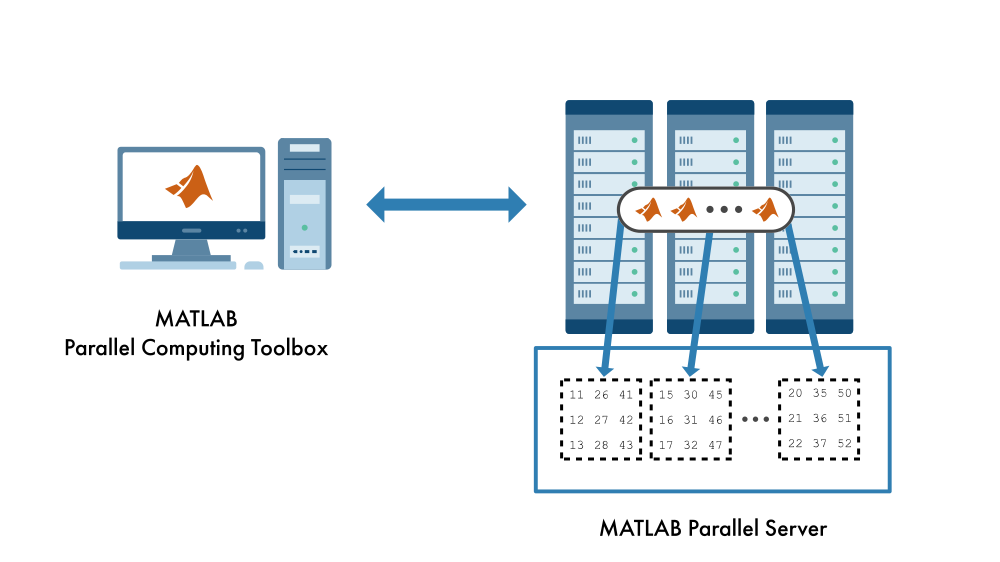
\includegraphics[width=0.8\textwidth]{../Immagini/Capitolo 2/ReferenceArchitecture.png}
    \caption{Architettura di riferimento per gli strumenti di calcolo parallelo in MATLAB. 
    \small{(Da \url{https://it.mathworks.com/products/matlab-parallel-server.html})}}
    \label{fig:ArchitetturaRiferimento}
\end{figure}

Giunti a questo punto, introduciamo le modalit\`a di esecuzione del software parallelo su un sistema multiprocessore supportate dall'ambiente MATLAB:
\begin{itemize}
    \item parallelizzazione implicita: alcune funzioni, se richiamate dal codice sorgente del programma, sfruttano le librerie di \textit{runtime} del linguaggio 
    in modo da essere eseguite su \textit{thread} distinti all'interno della stessa sessione;
    \item parallelizzazione esplicita: il carico di lavoro del programma viene automaticamente suddiviso in \textit{task} elementari, ciascuna delle quali viene 
    poi assegnata a un \textit{worker} per l'esecuzione.
\end{itemize}

\nocite{MathWorksParallelQuickStart}
\subsection{Il paradigma di programmazione parallela implicita}
I \textit{toolbox} di MATLAB sono dotati di un crescente numero di funzioni con supporto automatico al parallelismo, al fine di beneficiare di tutti 
i vantaggi propri dall'elaborazione parallela senza modificare il codice scritto per la versione seriale del programma, in accordo con i principi di design elencati 
nella sezione \ref{sec2.1.2}. 

Alcune funzioni, come \lstinline|mldivide| per la risoluzione di sistemi di equazioni lineari, vengono eseguite automaticamente in parallelo su \textit{thread} 
distinti se invocate dalla sessione principale di MATLAB. 

Ragionando sulla nostra architettura di riferimento, il parallelismo implicito viene attivato solo quando la funzione viene eseguita direttamente dal \textit{client}, 
mentre viene sconsigliato se l'esecuzione \'e a carico dei nodi del \textit{cluster} per evitare un parallelismo \enquote{annidato} che degraderebbe le prestazioni 
dell'intero sistema. \newline
In quest'ottica, possiamo notare come i progettisti del linguaggio abbiano pensato ai \textit{worker} come a unit\`a di elaborazione a singolo \textit{thread}.

Quando il \textit{client} incontra una funzione con supporto automatico al parallelismo nel codice sorgente del programma, avvia un \textit{parallel pool} per la 
sua esecuzione in parallelo. \newline
Un apposito profilo di configurazione determina le caratteristiche dell'ambiente di elaborazione parallela e, in particolare, PCT permette di scegliere tra i 
seguenti profili preimpostati:
\begin{itemize}
    \item \textit{Processes}: i \textit{worker} vengono attivati come processi indipendenti eseguiti dai \textit{core} fisici del calcolatore ospitante la sessione 
    principale di MATLAB.
    \item \textit{Threads}: i \textit{worker} sono eseguiti da \textit{thread} e non pi\`u da processi veri e propri. I vantaggi portati da questo ambiente 
    parallelo sono un minor uso di memoria, un basso costo di comunicazione tra i \textit{worker} e uno \textit{scheduling} delle attivit\`a particolarmente 
    performante, a scapito della disponibilit\`a di una ristretta gamma di funzioni con supporto al parallelismo su \textit{thread}.
\end{itemize}
Relativamente alla scelta del numero di \textit{worker} nell'ambiente \textit{Processes} \'e consigliato riservare un motore di calcolo per ogni \textit{core} 
fisico disponibile, ignorando la presenza di eventuali \textit{core} virtuali; infatti, questi ultimi condividono alcune risorse di calcolo all'interno dello 
stesso processore, tra cui la \textit{Floating Point Unit} (FPU), e poich\'e la maggior parte delle elaborazioni in MATLAB richiede l'esecuzione di operazioni 
aritmetiche in virgola mobile, limitare a uno il numero di \textit{worker} per unit\`a di esecuzione pu\`o aumentare la stabilit\`a del sistema. \newline 
L'unica eccezione \`e rappresentata dalle applicazioni \textit{data-intensive}, per le quali potrebbe essere conveniente portare il numero di \textit{worker} per 
\textit{core} fisico a due.

In ogni caso, un singolo \textit{parpool} a supporto della parallelizzazione implicita pu\`o contenere fino a 512 \textit{worker}, a prescindere dalle specifiche 
del calcolatore utilizzato.
\begin{figure}[htbp]
    \centering
    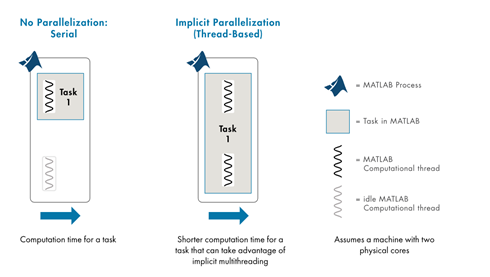
\includegraphics[width=0.8\textwidth]{../Immagini/Capitolo 2/ImplicitParallelization.png}
    \caption{Rappresentazione del modello di parallelizzazione implicita di MATLAB su un sistema \textit{dual-core}
    \small{(Da \url{https://it.mathworks.com/discovery/matlab-multicore.html})}}
    \label{fig:ParallelismoImplicito}
\end{figure}\newline
Se una funzione non include il supporto automatico al parallelimo, possiamo trasferire l'esecuzione del programma a una \textit{workstation}, in modo da beneficiare 
dello \textit{speedup} offerto da un sistema con maggiore capacit\`a di calcolo, oppure possiamo utilizzare il paradigma di programmazione parallela esplicita 
supportato dal \textit{Parallel Computing Toolbox}.

\subsection{Il paradigma di programmazione parallela esplicita}

Il modello di programmazione parallela esplicita esposto dal \textit{Parallel Computing Toolbox} si fonda sull'esistenza di costrutti di programmazione 
parallela a diversi livelli di astrazione, di cui i programmatori si possono avvalere durante la stesura di programmi a esecuzione parallela.\newline
Il meccanismo a bassissimo livello presente per la scrittura di programmi a elaborazione parallela \`e basato sullo scambio di messaggi tra i \textit{worker} 
appertenenti a un medesimo \textit{parallel pool}, ma lo sviluppo di programmi secondo questo approccio viene spesso criticato, essendo considerato l'equivalente del linguaggio 
Assembly per la programmazione parallela.\newline
Per agevolare la scrittura di software parallelo, alcuni costrutti di programmazione di alto livello sono introdotti nel linguaggio, aumentando il livello di 
astrazione del codice scritto e consentendo ai programmatori di scrivere algoritmi paralleli in modo simile alle loro controparti seriali.

Un esempio di costrutto di alto livello per la programmazione parallela \`e incarnato dagli \textit{array} 
\footnote{Nel gergo impiegato da MATLAB, la parola \textit{array} \`e un termine universale per riferirsi a vettori colonna, vettori riga e matrici} 
distribuiti, strutture dati il cui contenuto viene partizionato tra \textit{worker} diversi.\newline
L'impiego di \textit{array} distribuiti permette di memorizzare strutture dati di dimensioni tali da non poter essere contenute nella memoria centrale di un 
singolo calcolatore, sfruttando la capacit\`a di memoria combinata offerta dai nodi del \textit{cluster}.

Gli \textit{array} distribuiti possono contenere dati di qualsiasi tipo e supportano la distribuzione dei loro elementi tra i worker lungo una dimensione, ovvero 
per riga oppure per colonna; a questo proposito, dobbiamo precisare che l'utente ha la possibilit\`a di definire distribuzioni dei dati alternative e che, 
molto spesso, il partizionamento degli elementi tra le unit\`a di lavoro viene modificato implicitamente dall'esecuzione di certe operazioni, 
come \lstinline|gather| una funzione utile a trasferire un \textit{array} distribuito nello spazio di lavoro del \textit{client}.

Un ulteriore vantaggio derivante dall'uso degli \textit{array} distribuiti \`e l'assenza di differenze sintattiche per l'accesso agli elementi rispetto ai 
tradizionali \textit{array}; l'infrastruttura sottostante garantisce in ogni momento una dsitribuzione dei dati idonea all'esecuzione delle operazioni 
richieste dall'utente.\newline
Questa ampia possibilit\`a di manovra lasciata al programmatore potrebbe introdurre consistenti \textit{overhead} di comunicazione tra i \textit{worker}, 
ma sappiamo che la programmabilit\`a rappresenta l'obiettivo di design prioritario nel processo di parallelizzazione di MATLAB, perfino a scapito delle prestazioni.

Centinaia di funzioni MATLAB native, e altrettante presenti nei \textit{toolbox} sviluppate dalla \textit{community}, sono state progettate per adattare il 
loro comportamento alla ricezione di parametri distribuiti in ingresso.\newline
Ad esempio, MATLAB prevede un ampio insieme di funzioni parallele per l'algebra lineare che operano su \textit{array} distribuiti, implementate a partire dalle \textit{routine} definite dalla libreria di algebra lineare numerica ScaLAPACK.